\documentclass[11pt]{article}
\usepackage[english]{babel}
\usepackage{inputenc}
\usepackage{multicol}
\usepackage{flushend}
\usepackage{fullpage}
\usepackage{epsfig}
\usepackage{caption}
\captionsetup[table]{labelsep=period}
\usepackage{multirow}
\usepackage{mathtools}
\usepackage{xcolor}
\DeclarePairedDelimiter{\ceil}{\lceil}{\rceil}

\topmargin=-0.2in
\textheight=9.5in

\pagestyle{empty}

\begin{document}

\centerline{CSCE 614 (Fall 2020) \hfill Uwacu and Elsheimy}
\medskip
\centerline{\bf Computer Architecture}
\medskip

\centerline{\bf  Project report: }

\bigskip

\centerline{\bf Exploring Predictive Replacement Policies for Instruction Cache and Branch Target Buffer}

\bigskip

\centerline{\bf Diane Uwacu and Fatmaelzahraa Elsheimy}

\bigskip

\begin{abstract}
Many of the new-era processors support fetching instructions with instruction cache and branch target buffer. I-Cache and branch target buffer have limited capacities and
therefore, different types of replacement policies are being explored to reduce the misses in I-cache and BTB. In this project, we implement a new policy Global History Reuse 
Prediction (GHRP), a replacement policy that uses the history of previous instructions and behaviour predict and evict dead blocks. GHRP is implemented in the main paper using
Championship Branch Prediction simulator, but we try to implement it using Zsim to test the easiness of implementing the new policy in different simulators. GHRP’s performance
is compared against the famous policy LRU (Least recently used) and SRRIP(static re-reference interval prediction). Using Championship simulator, GHRP reduces the I-cache misses (MPKI) by 18% 
over LRU policy on a 662 industrial workloads. In Zsim, LRU data is collected over PARSEC benchmark and the results are speculated from the Championship results.
\end{abstract}

\section{Introduction} 
\label{sec:introduction}

Current processors need efficient instruction fetch for high performance. There are two main structures that the processor rely on for efficient fetching: I-cache and branch
target buffer. The instruction cache (I-cache) keeps record of recently used instructions, and the branch target buffer (BTB) caches targets of previously taken branches.
Therefore, the I-cache helps in improving instruction throughput and latency. Branch target buffer improves latency because of branch target-recomputation. This paper [3] 
explores efficient replacement policies at the I-cache and BTB levels. Samira et-al introduces a new idea for policy replacement called Graph History Reuse Prediction. This 
algorithm is based on the history of past instruction addresses and behaviour in order to predict dead blocks in an efficient way. Predicting dead blocks is very important as
they free up space for other blocks that might be used in the future. A block is said to be dead if it is not going to be used before eviction. A block is said to be live if it 
is going to be used before eviction. Samira et-al have done a survey on the current implemented policies such as LRU, SSRIP..etc and tried to find a better policy. Most of the
work on _cache optimization focused on instruction prefetching and block reordering. Many of these solutions didn’t lead to good  outcome as it resulted in large overhead or 
high MPKI. Similarly, most of the work on BTB optimization focused on the design structure or using different replacement policy. Again, the results weren’t that satisfactory.
Samira et-al first, tried to apply PC-based predictor that uses set-sampling for Cache behavior generalization, however, when being applied on I-cache and BTB, they haven’t 
seen prominent results and hence, this idea was discarded. On the other side,  based on the survey done over all current replacement policies, they noted that that sequences of
recently accessed instructions correlate with the likelihood of block reuse. Their proposes policy results in a prominent improvement in cache efficiency and overall 
performance. They evaluated seven recent replacement policies and compared them based on average MPKI values. While, Samira et al applied their policy on Championship 
simulator. We have tried applying it on Zsim to test the ease of implementation of the policies in different simulators and compare the results using different benchmark; 
PARSEC.


\section{Background}
\label{sec:background}


\section{Work Description}
\label{sec:proposed}

\section{Evaluation}
\label{sec:timeline}

\subsection{Experimental Setup}

\subsection{Experimental Results and Discussion}

\begin{figure}[h]
	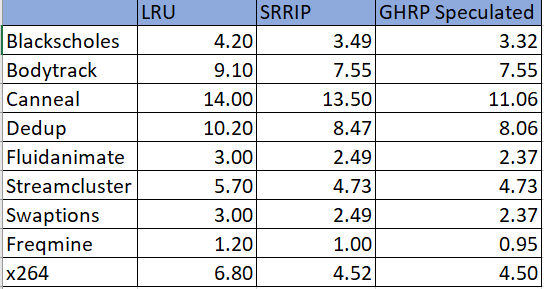
\includegraphics[width=1\textwidth]{MPKI1.PNG}
	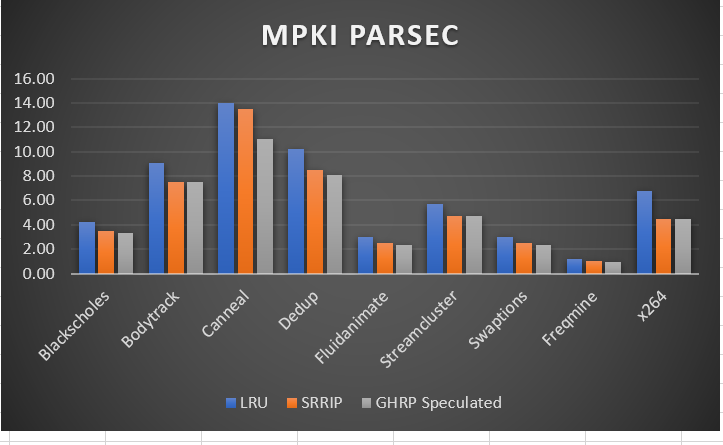
\includegraphics[width=1\textwidth]{MPKI2.PNG}
\end{figure}

\section{Conslusion and Future Work}

{%\scriptsize
	\bibliographystyle{abbrv}
	\bibliography{references}
	}

\end{document}



